\chapter{Dise\~no del Sistema}
\begin{indentar}
\end{indentar}

\section{Dise\~no de la Arquitectura del Sistema}
\begin{indentar}
Debido al requerimiento no funcional, de separar el Sistema actual \textbf{AppVlir8} en dos productos, uno en la Administraci\'on de Eventos Cient\'ificos y el otro en la Administraci\'on de Grupos de Investigaci\'on, el dise\~no de la Arquitectura fue concebido de la siguiente manera.

\begin{figure}
  \centering
    {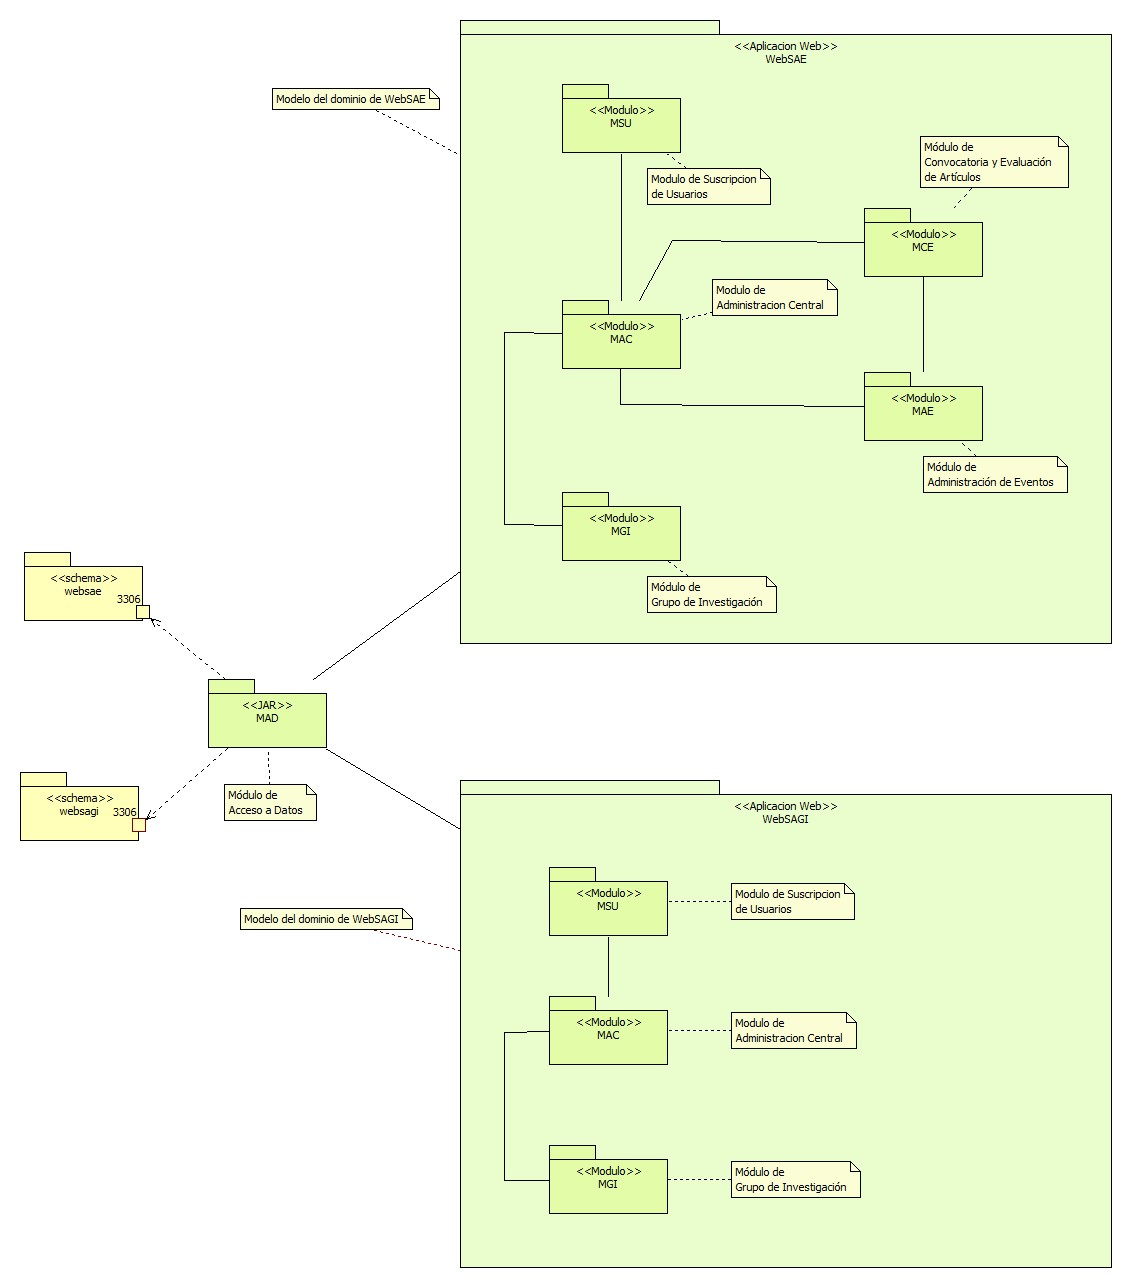
\includegraphics[width=1.0\textwidth]{images/websaegi-arquitectura.eps}}
  \caption{Dise\~no de Arquitectura del Sistema de Administraci\'on de Eventos y Grupos Cient\'ificos.}
  \label{websaegi:arquitectura}
\end{figure}

La definici\'on de la anterior imagen~\ref{websaegi:arquitectura}, es concebida como dos sistemas independientes que utilizan otro m\'odulo no mencionado al inicio, debido a que este m\'odulo no pertenece al dominio, si no que surge en el dise\~no de la Arquitectura, este m\'odulo fue llamado MAD (M\'odulo de Acceso a Datos)\footnote{Es importante recalcar que este m\'odulo fue ideado por la Srta. Diana Crespo -jefa de Sistemas en Molemotor-, llam\'andolo inicialmente ADA, por el dise\~no portable de \'este, se lo adecu\'o a MySQL -ya que fue implementado para que trabajase con la Base de Datos SQL Server 2000- y para que pueda trabajar con WebSAE y WebSAGI, las bases de datos de la Administraci\'on de Eventos y de los Grupos de Investigaci\'on, respectivamente.} este framework, permite a los Eventos la conexi\'on a la Base de Datos de los Grupos de Investigaci\'on y viceverza.
\end{indentar}

\subsection{Dise\~no Arquitect\'onico}
\begin{indentar}
En nuestro caso, s\'olo se implement\'o el Sistema Web de Administraci\'on de Eventos Cient\'ificos, tambi\'en denominado \textbf{WebSAE}, el mismo que se muestra a continuaci\'on \ref{websae:arquitectura}, que ser\'ia tan s\'olo una de las partes antes mostrada.

\begin{landscape}
\begin{figure}
  \centering
    {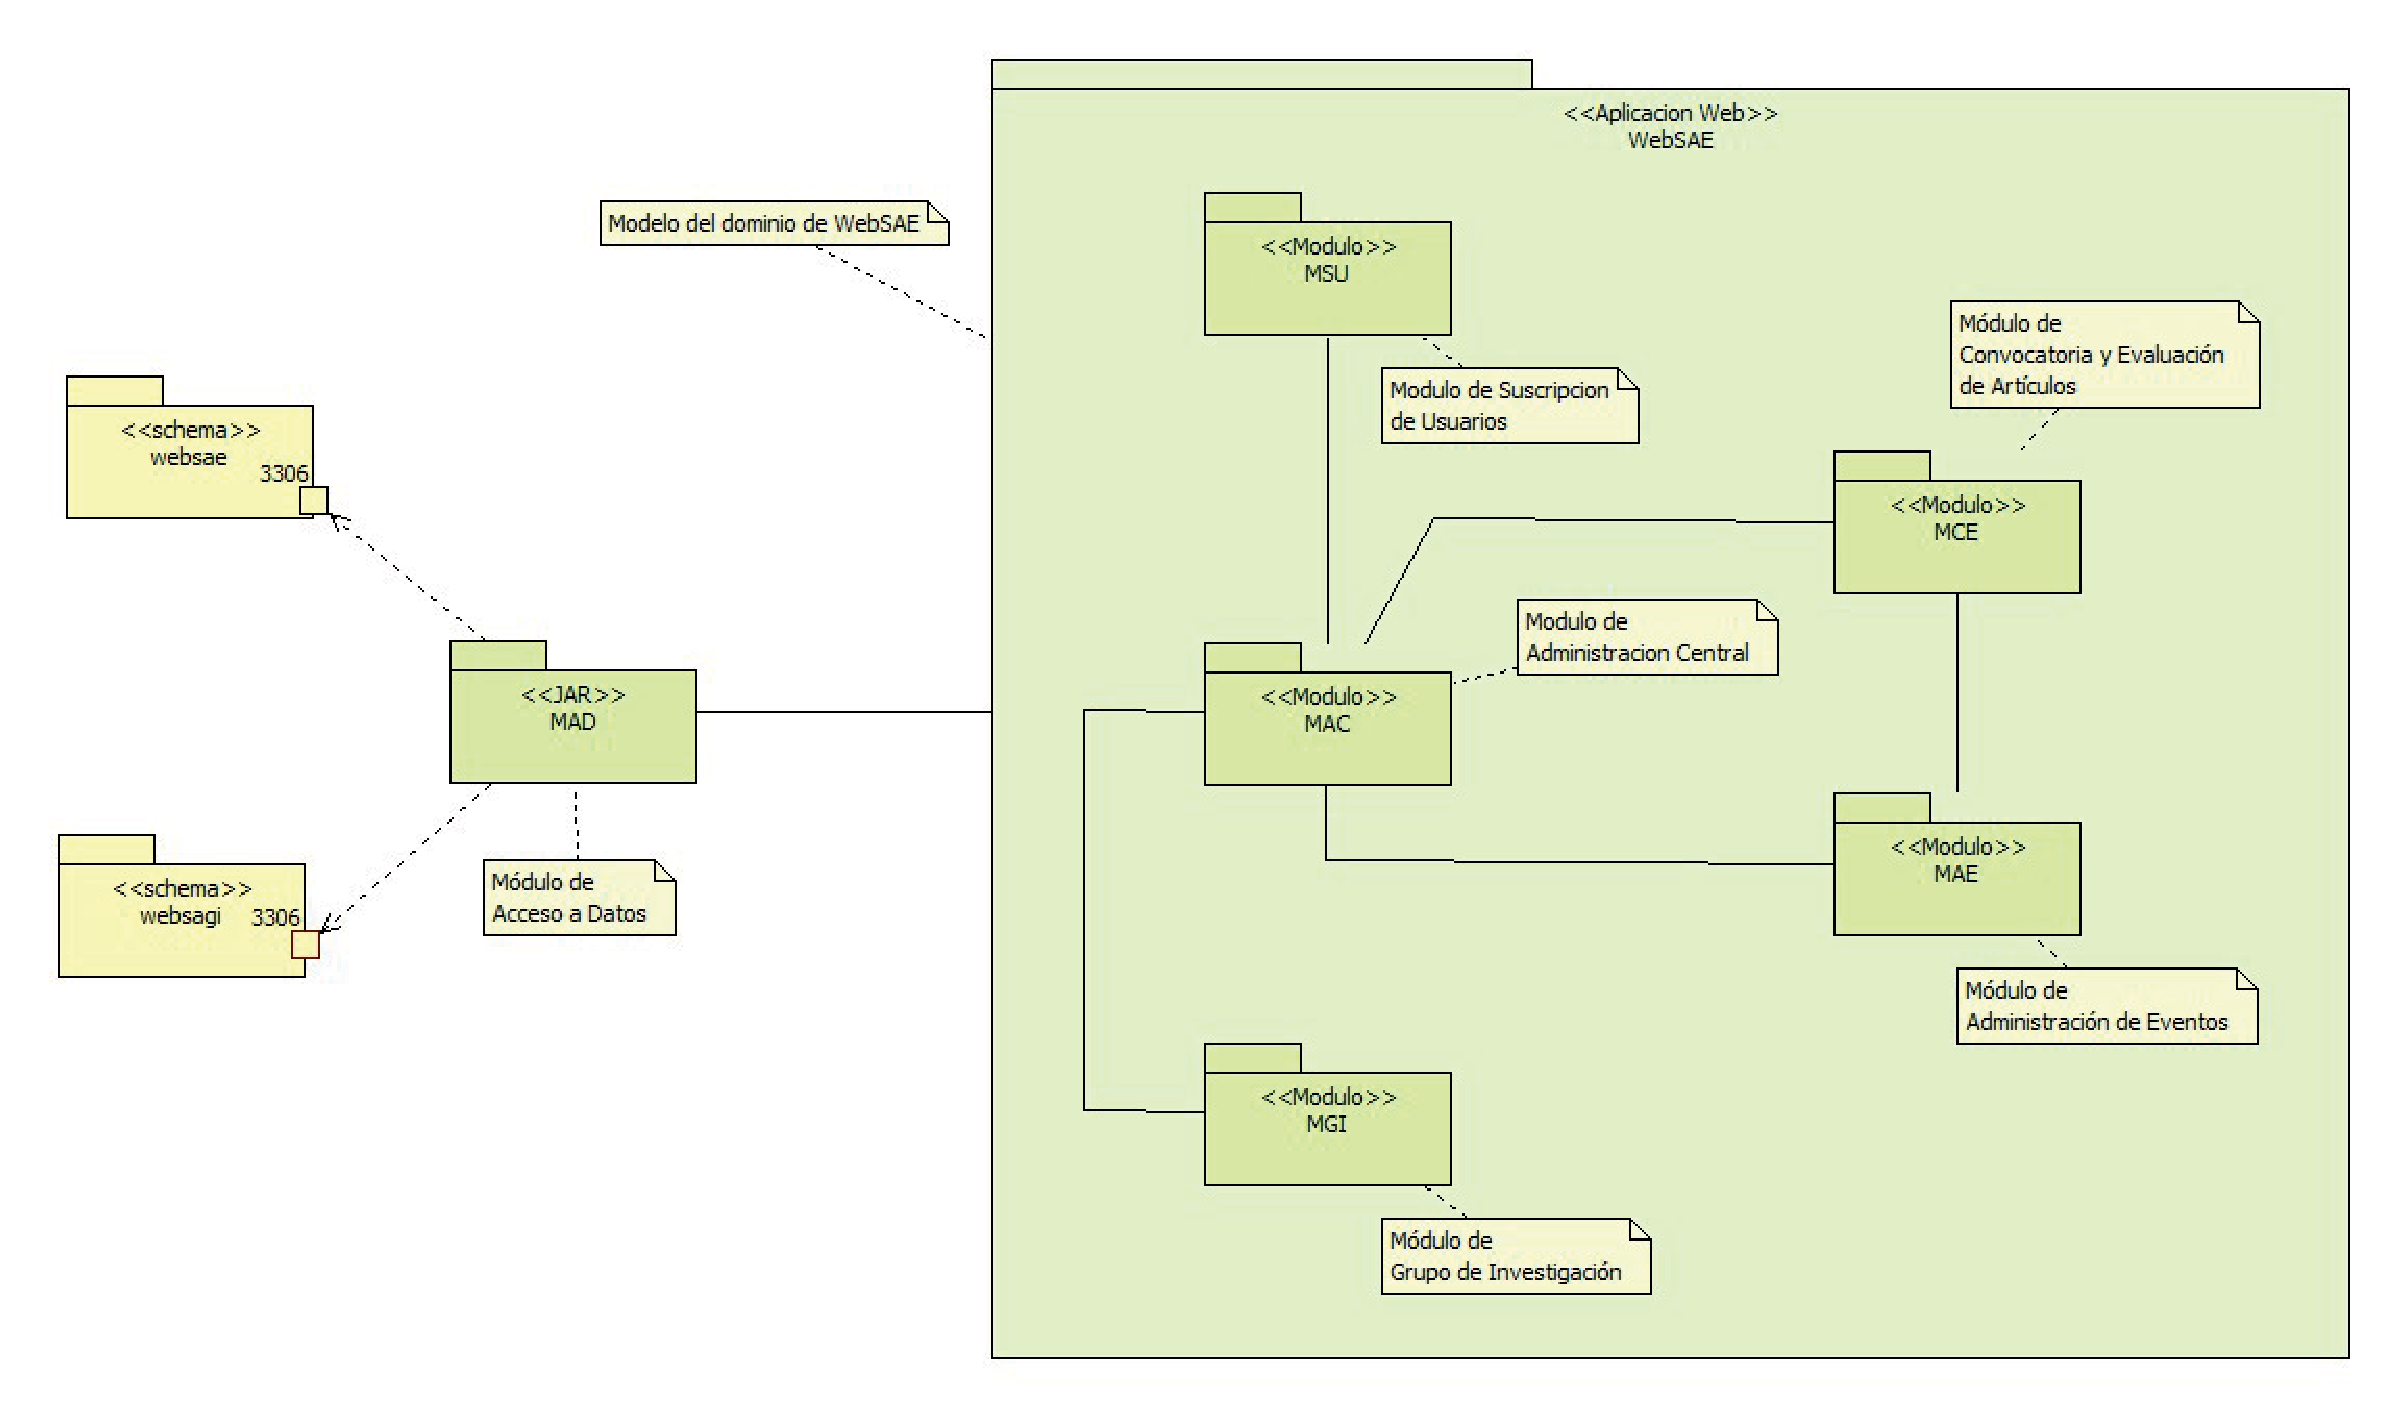
\includegraphics[width=1.4\textwidth]{images/websae-arquitectura.eps}}
  \caption{Dise\~no de la Arquitectura del Sistema de Administraci\'on de Eventos.}
  \label{websae:arquitectura}
\end{figure}
\end{landscape}

\end{indentar}

\subsection{M\'odulos del Sistema}
\begin{indentar}
\end{indentar}

\subsection{Arquitectura basada en patrones de dise\~no}
\begin{indentar}
\end{indentar}

\section{Diagrama de Clases del Sistema}
\begin{indentar}
\end{indentar}

\section{Modelo l\'ogico de la Base de Datos}
\begin{indentar}
\end{indentar}
